\documentclass{scrartcl}
\usepackage[utf8]{inputenc}
\usepackage{graphicx}
\usepackage{indentfirst}
\setcounter{secnumdepth}{0}

\title{Poupon: Technical Report, Phase 2}
\subtitle{CS 373 Software Engineering, Fall 2017}
\author{Sarah Wang, William Xu, Logan Zartman, Christian Carroll, Zach Burky}
\date{October 26, 2017}

\begin{document}

    \maketitle

    \tableofcontents

    \newpage
    \section{Motivation}\label{sec:motivation}
    \indent
    Music has always been a dominant force in the past centuries.
    Encompassing many different genres and cultures, music has provided another means in which others can learn about themselves or others.
    While the music industry has experienced a 40\% decline globally in the last two decades, with the release of portable audio players and streaming services such as Pandora, Spotify, and Apple Music, the music industry has seen amazing growth.
    With a nearly 15 billion and rising global revenue this past year, the music industry's revival seems all but impossible.
    Additionally, as the Information Age and Internet of Things (IoT) phenomenon comes into full swing, we've seen the music industry blossom as never been seen before.

    With streaming services in full bloom, it's rare to meet a classmate, friend, or family member who hasn't heard of Spotify, Apple Music, Pandora, or any of the major music streaming companies.
    In fact, streaming services are so intertwined in this age with the modern music industry that many up and coming artists have had their first albums, mixtapes, and songs hosted on one or more of these platforms (such as Bandcamp or SoundCloud).
    Gone are the original days of getting the attention of producers and record labels through forced encounters or even snail mail, in many ways, like many other IoT and Data companies, the music industry has evolved from a previously offline process to a very entrenched, online process.
    Viral videos and views are the way that much of today's stars have had their humble beginnings.
    Additionally, shows like American Idol and The Voice have used the power of mobile phones to full use, combining the IoT phenomenon that we're experiencing in order to discover new stars that we can fervorously follow.

    Given the vast number of genres available at our disposal through streaming sites, it's difficult to understand why we would decide to home in or focus on only hip-hop/R\&B. However, for many of us, these two genres encompassed much of our childhood and was a solid foundation for many of the youth in our generation.
    Songs from Usher's earlier albums like Confessions to even Kendrick Lamar's newest album DAMN., have played anywhere from the crowded cities of New York to the quiet suburbs of cities like Plano.
    Additionally, hip-hop/R\&B's rich intertwined history in our country's own history naturally makes it a great genre to focus on and potentially present to others.
    All in all, hip-hop/R\&B's ability to connect others despite background, social standing, and culture makes it an excellent medium to focus on for our app.
    It's ability to transcend boundaries and relatability make for a great conversation starter, providing a great avenue for others to meet each other.

    On a related note, the name of our domain (poupon.me) comes from the dijon mustard, Grey Poupon, which has been mentioned in numerous popular songs in the past decades by artists like Kanye West and Jay-Z.
    The brand's status of luxury, style, and class, as well as its easiness of use in rhyme, make it a natural inclusion in most songs.
    For us, it was no question to incorporate it into our site, built to spread, educate, and introduce Hip-Hop and R\&B to others.

    \section{Use Cases}\label{sec:useCases}
    \indent As mentioned earlier, poupon.me's primary use case is to introduce Hip-Hop and R\&B to all listeners.
    Whether they're new listeners or "experienced" listeners, our website is aimed at helping listeners experience Hip-Hop in a different way than the "shuffle" button on streaming services such as Spotify.
    Our site is dedicated to seeing Hip-Hop and R\&B in different ways;
    By classifying artists by their most successful albums, city, or even their top acclaimed songs, we can introduce a more introspective way of listening.
    For example, by viewing Artists and even Albums by Cities, we can help listeners find related Artists or even styles, dividing cities into different sub-genres much like the "East Coast vs West Coast" rivalry of the mid to late 1990s.
    The news tab also can help introduce the newest, trending songs to listeners, without the need of going through other websites or being bombarded by their friends.
    In short, our website provides an additional view of listening to hip-hop and R\&B on top of the original methods of scrolling through songs and albums.

    While our original attention is for poupon.me to contain information on only Hip-Hop and R\&B, the structure of the API allows for other genres and even single albums, artists, cities, and articles to be added without any worries.

    \section{RESTful API}\label{sec:restfulApi}
    The first API that we used was the Spotify API: \begin{verbatim}
                                                        https://developer.spotify.com/web-api/endpoint-reference/
    \end{verbatim}

    While intimidating at first, making use of the Spotify API became much easier as we familiarized ourselves with Spotify's Web API over the course of the week.
    Spotify provides excellent documentation for its own API and has a wide variety of different calls that we can call to receive the information we need.
    In fact, there were some calls like "GET Audio Analysis for Track" that provided some ideas for future iterations on top of our site.
    All in all, Spotify's API was an excellent resource for pulling Album, Artist, and Song information and gave us inspiration for potential additions to our site.

    Although the API was well documented and simple, our first major problem with working with the Spotify API was acquiring an authorization code/access token for using the API.
    Thankfully, Spotify had an authorization guide that we followed in order to resolve this.
    For generating our API requests, We debated over using Flask, cURL, or a third party GUI like Postman or the Insomnia REST Client.
    For now, the team decided to use a third party GUI when creating the persistence layer, but we did not decide on which specific app to use yet.
    Additionally, the team wanted to use Flask to serve additional requests to potentially pull new data points that were not in our persistence layer.
    Since the persistence layer is not necessary for the first sprint, we decided to use a combination of cURL and the provided web tool in Spotify's developer portal and finalize the structure of the persistence layer at a later iteration of our project.

    Our second problem with using the API was that Spotify stored much of their information through unique IDs.
    Rather than being able to use an API call with an artist's name, we had to first use the search-item endpoint to determine the unique ID, and then use another API call to get the information that we needed.

    As of now, the API Calls specifically used were the following:

    \begin{itemize}
        \item This is the API Call that we use to search for the unique IDs of each of the following fields:
        \begin{verbatim}
            GET https://api.spotify.com/v1/search
        \end{verbatim}

        \item This is the API Call to retrieve album information from the API:
        \begin{verbatim}
            GET https://api.spotify.com/v1/albums/{id}
        \end{verbatim}

        \item This is the API Call to retrieve artist information from the API:
        \begin{verbatim}
            GET https://api.spotify.com/v1/artists/{id}
        \end{verbatim}

        \item This is the API Call to retrieve related artist information:
        \begin{verbatim}
            GET https://api.spotify.com/v1/artists/{id}/related-artists
        \end{verbatim}
    \end{itemize}

    \noindent
    The second API that we used was the PRAW Reddit API:
    \begin{verbatim}
        https://github.com/reddit/reddit/wiki/API
    \end{verbatim}

    \noindent
    We used the PRAW (Python Reddit API Wrapper) in order to easily scrape data about articles:
    \begin{verbatim}
        http://praw.readthedocs.io/en/v3.6.1/pages/getting_started.html
    \end{verbatim}

    So far, we used the wrapper to write a script to pull a few Reddit posts to serve as examples.
    We wrote a script that went to the reddit.com/r/hiphopheads top posts of all time.
    The script then scraped articles that related to the artists we have on our website at this point.

    In the future, we will explore whether we want to use the Reddit API directly or continue using PRAW.
    We will need to pull many more articles and we will have many more artists in our database, which may make it easier to just use the Reddit API.\\

    \noindent
    The third (and final so far) API that we will use is the US Census Bureau API:
    \begin{verbatim}
        https://api.census.gov/data.html
    \end{verbatim}

    This implementation is more vague, as the sheer amount of data sets that the Census contains is abnormally large, and the amount that we want to take from it (accurate population values, as of right now) is very limited> Additionally, as we're pre-loading our database with around 100 instances of each model for the second phase, this will be something we complete in the third phase.

    \section{Models}\label{sec:models}
    We have chosen four models to use in our site: artists, albums, articles, and cities.

    \subsection{Artist}\label{subsec:artist}
    An artist is a person or group that has released music.
    This model contains personal information about an artist as well as information about the music they have released.
    This information is scraped using the Spotify API.\\

    Attributes:
    \begin{itemize}
        \item Name
        \item Genres
        \item Albums
        \item Image
        \item Related Artists
    \end{itemize}

    If we desired, there's obviously any number of attributes that could be added to an artist - cities, trending news, age, photographs, embedded media, links to songs/albums, etc.
    However, in the earliest iteration of the site, we are keeping it so that the number of attributes connected to any given node is minimal, so as to avoid confusion when learning how to integrate all the different pieces that combine to make a functional stack.
    Once we have a more functional working product (and practical understanding of web dev), it will be a lot more feasible to consider expanding the models' attributes.

    \subsection{Album}\label{subsec:album}
    An album is a collection of songs released as a group.
    This model contains a list of songs as well as metadata about the album.
    This information is scraped using the Spotify API.\\

    Attributes:
    \begin{itemize}
        \item Name
        \item Artists
        \item Release Date
        \item Label
        \item Cover Art
        \item Tracklist
    \end{itemize}

    \subsubsection{Track}
    We have a secondary model under albums, so we can more easily define the tracklist.
    We only store name and length, as well as a Spotify link.
    This is also scraped using the Spotify API.\\

    Attributes:
    \begin{itemize}
        \item Name
        \item Track number
        \item Spotify link
        \item Album
    \end{itemize}

    \subsection{Article}\label{subsec:article}
    An article contains information about a hip hop related news article and the artists mentioned in the article.
    We pull our articles from reddit.com/r/hiphopheads using the Reddit API.\\

    Attributes:
    \begin{itemize}
        \item Title
        \item Score (Reddit upvotes)
        \item Number of comments
        \item URL
        \item Artists
    \end{itemize}

    \subsection{City}\label{subsec:city}
    The city model contains general information about a city in addition to hip hop specific information.
    This information is pulled from the census data.\\

    Attributes:
    \begin{itemize}
        \item Name
        \item State
        \item Population
        \item Artists
        \item Coordinates
    \end{itemize}

    \section{Database}\label{sec:database}
    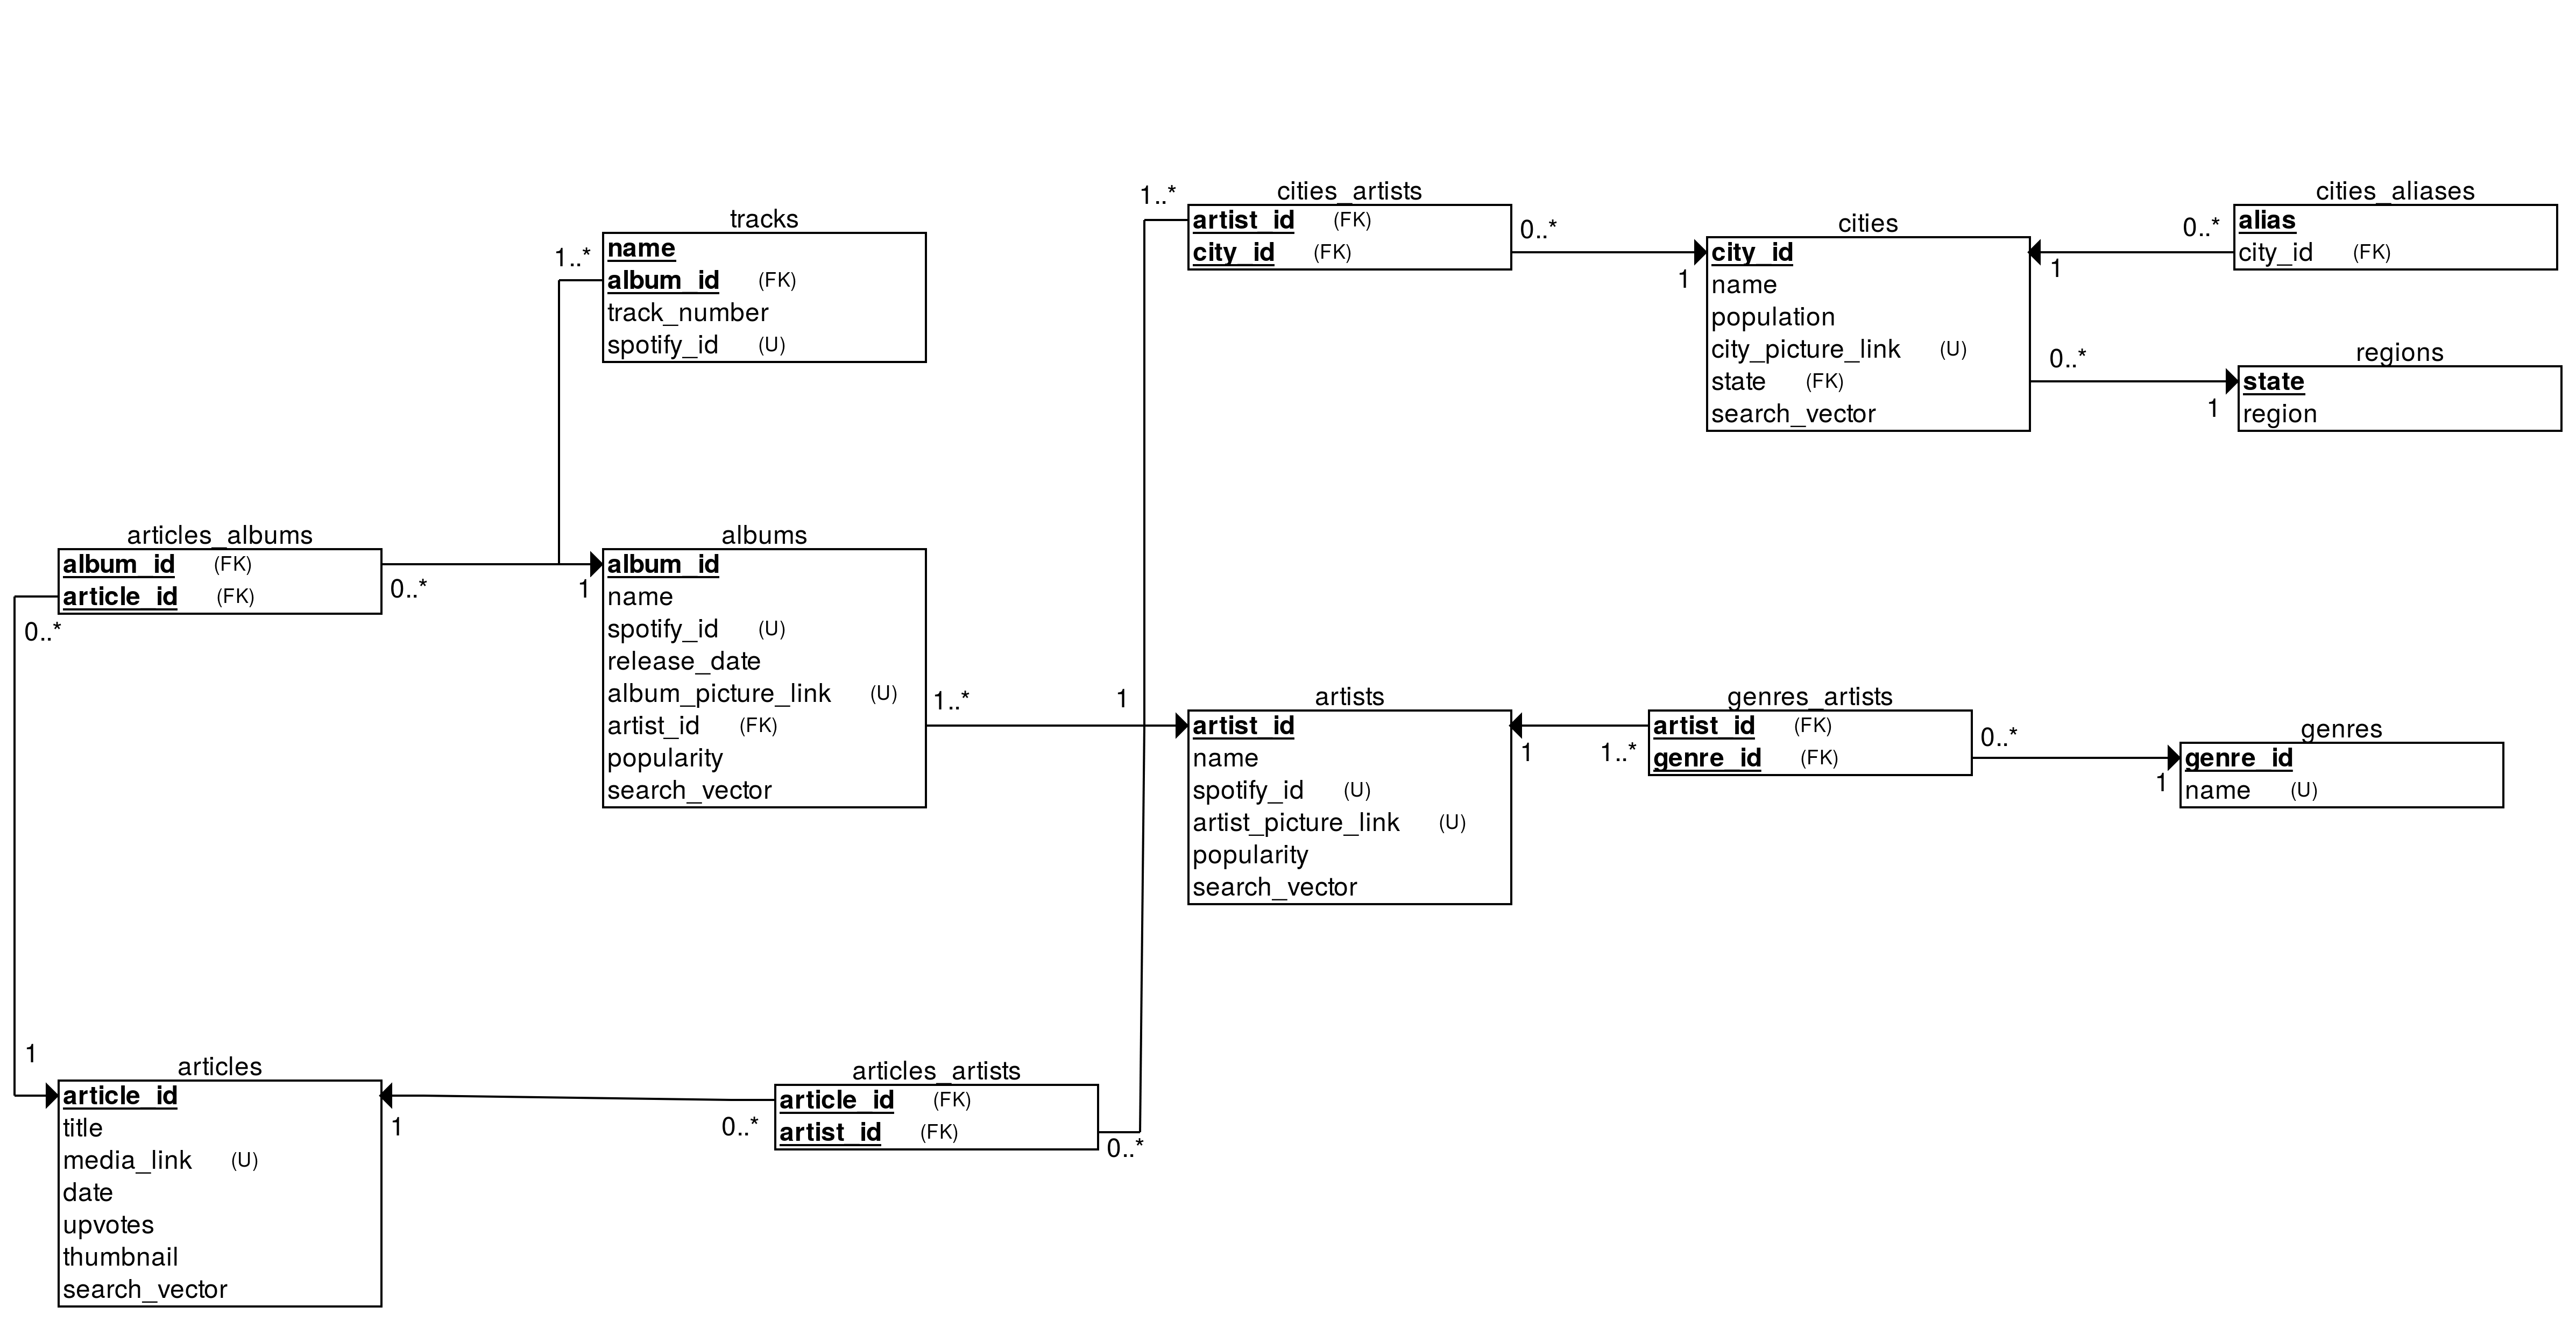
\includegraphics[width=1\textwidth]{uml}
    \textit{Note: for a more high-resolution depiction of the UML, please see the attached 'uml.png'}\\

    Our database is crucial to the function of our website.
    Rather than having React make calls to external APIs every time we want to display data on artists, albums, articles, or cities, and then having to set up rules to be able to legibly parse those calls on the fly, we designed a database schema that we can use to reliably store and retrieve data from a local source in a consistent manner.

    The first step to designing this schema was to identify the four classes based on our four models - artists, albums, articles, and cities.
    We identified attributes for these models, using a surrogate ID for artists, albums, and cities (which was actually a Spotify external key for artists and albums, and possibly a PRAW external key for articles).
    From there, we identified a few supplementary tables that we anticipate being useful, such as tracks for albums, genres for albums and artists, regions for cities, and aliases for cities (for future use in the lyrical analysis portion of Poupon).

    Now, we run into the problem of connecting the databases.
    If we were to include a foreign key in every table so that each table could communicate with the other, we would introduce a massive amount of inefficiency, as well as making our schema harder to understand.
    Instead, we introduced relational table, such as news/albums (for relating news articles to specific albums), news/artists (the same for articles and artists they mention), genres/artists (for connecting predetermined genres to artists), and cities/artists (to connect the places an artist might be related to).
    By creating these tables, we retain full functionality, as each table can query another by using a series of select statements, and we have the added benefit of having small tables where each row can be guaranteed as unique.\\

    We've implemented this database using SQLAlchemy.
    This allows us to create Python that can then be interpreted into SQL statements that can be fed to GCP CloudSQL for use in our PostgreSQL database.
    More details as to the implementation can be found inside of the tools section on SQLAlchemy.
    This has been especially useful, as it has allowed us to generalize our database's tables into class tables, which can be clearly defined using parameters for primary keys, foreign keys, and the like.
    Additionally, it makes constructing relational tables as easy as defining the tables, and adding secondary attributes in the tables they relate to.

    We have a few small design decisions, mainly concerning the size of the database.
    We'll be predefining on the order of 100 artists, 200 albums, 10 cities, and a variable number of articles for this second stage of the project, so as to limit the number of things that can go wrong at any one time - it should be said, however, that we do intend to implement actual automated external calling across the board in the next phase - Christian has already set that up for GitHub and Trello, so it should just be a matter of figuring out the correct ingest procedure.

    DISCLAIMER: as of right now, the table for city aliases is unused and unpopulated - we plan to implement this alongside our text analysis of news titles for mentions of instances of other models.

    \section{Tools}\label{sec:tools}

    \subsection{make}\label{subsec:make}
    GNU Make enables us to create recipes for simple, automated builds of source and non-source files.
    Make recipes are defined in a Makefile in the top level directory of our repository.
    We handle packaging our web app with the Webpack setup provided by create-react-app.
    We do, however, use make to allow us to easily deploy to Google Cloud Platform, test our app locally, and even install necessary build tools.

    \subsection{git}\label{subsec:git}
    We use a git repository hosted on GitHub to provide version control.
    Using a centralized version control system enables us to work in parallel on the same files and merge our edits-often automatically.
    Hosting our project in a git repository also allows us to revert changes that cause new bugs, or even inspect older versions of the code on our machines.
    Git ensures that we never lose work, and never make destructive edits.

    \subsection{Bootstrap}\label{subsec:bootstrap}
    Bootstrap is a CSS framework that provides a "responsive" layout system-that is, the layout scales and rearranges automatically to fit various screen sizes and device types.
    Bootstrap also helps to normalize page styles across various browsers, and provides a selection of components that can be used in our web app.
    Components include things such as buttons, dialogs, navigation bars, and cards for grouping content.
    Bootstrap allows us to design a responsive layout by setting up a 12-column grid, and specifying how many columns should be occupied by a given element on a device with a given screen size.
    For example, a card might have a width of 4 columns on large displays but the full 12 columns on small displays.
    A full-width banner, on the other hand, would have a size of 12 columns on all displays.

    \subsection{React}\label{subsec:react}
    React is a component-based, declarative JavaScript framework for building UIs.
    React components are essentially templates that allow the programmer to render data into HTML to present to the user.
    This data can be retrieved dynamically and be used to update components entirely on the client side-in our setup, no rendering occurs on the server.
    However, React is distinct from some template frameworks in that React components are written in a superset of JavaScript called JSX.
    JSX enables HTML templates and JavaScript logic to be written in the same file.
    This means that there is no unnecessary shoehorning of data and logic into HTML-based templates.

    \subsection{create-react-app}\label{subsec:create-react-app}
    create-react-app automates the process of creating the skeleton for a React web app.
    Additionally, it automatically configures Webpack to build an optimized production version of our React website.
    create-react-app enables us to use JSX and ES6 syntax.
    It even provides a web server that lints for errors and allows us to test our app locally.

    \subsection{Flask}\label{subsec:flask}
    Flask is a lightweight web framework for Python.
    Eventually, we will use Flask to provide our API endpoints.
    Our Flask-based backend will be responsible for querying our database, querying external REST APIs to collect data, and responding to requests to our API endpoints at poupon.me/api.

    \subsection{Nifi}\label{subsec:nifi}
    Apache NiFi is web-based user interface designed to process and distribute data.
    From their website, Nifi is described as a reliable system that supports scalable data routing, transformation, and system mediation logic.
    We use Nifi as an essential part of our ETL (Extract, Transform, Load) layer.
    Specifically, we clean the data we pull from API sources like the SpotifyAPI through our scripts and only extract the relevant data attributes that are needed in our database.
    After extracting the relevant data, we package the data into a stream of JSON objects for loading into our database.

    \subsection{JQ}\label{subsec:jq}
    JQ is a lightweight and flexible command-line JSON processor.
    Like sed, awk, and grep is for text, jq is the same way for JSON data, allowing us to transform JSON data with relative ease on the command line without having to write our own scripts to do so.
    We use JQ to transform the JSON object stream created from our NiFi pipeline into a JSON object array that our python scripts use to insert our data in to the PostGRESQL.

    \subsection{SQLAlchemy}\label{subsec:sqlalchemy}
    SQLAlchemy represents the main new tool we've implemented.
    Essentially, it acts a Python framework that allows you to construct SQL statements in a manner that is understandable from the Python level.
    As an example, if we wanted to have a table named 'artists' (which we do) with an attribute 'artist\_id' that acted as a integer primary key, and an attribute 'spotify\_link' that is unique and of variable length, we could implement that in Python/SQLAlchemy as follows:

    \begin{verbatim}
        from sqlalchemy.ext.declarative import declarative_base
        from sqlalchemy import Column, Integer, String

        Base = declarative_base()

        class Artist(Base):
        __tablename__ = "artists"

        artist_id = Column(Integer, primary_key=True, nullable=False)
        spotify_link = DColumn(String, unique=True, nullable=False)
    \end{verbatim}

    This would be equivalent to a SQL statement as follows:

    \begin{verbatim}
        CREATE TABLE artists
        (
        artist_id INT NOT NULL,
        spotify_link VARCHAR NOT NULL,
        PRIMARY KEY (artist_id),
        UNIQUE (spotify_link),
        );
    \end{verbatim}

    \subsection{Postman}\label{subsec:postman}
    Postman is a REST Client similar to Insomnia.
    Much like Insomnia, it provides the same intuitive UI design and the same cross-platform compatibility.
    The difference between Postman and Insomnia are minor UI design decisions;
    therefore, using one or the other is up to team/personal preference.
    We elected to use Python, due to William's familiarity with it.

    \subsection{Docker}\label{subsec:docker}
    Docker is a utility that can be used to spin up pre-defined containers for testing and deployment.
    We use Docker back-end testing and local deployment, but for deployment to the production version of Poupon, we elected not to.
    Due to numerous problems with how Docker interacted with GCP, we thought it would better / more efficient to not use it on the deployed side of the site.

    \section{Hosting}\label{sec:hosting}
    Our web app is hosted on Google Cloud Platform.
    We use Google App Engine to simplify the process of running our Flask backend and serving the static files for our React web app.
    We use the GCP web console to manage our app and the GCP command line tools to deploy it from our local machines.
    We create a small app.yaml configuration file to specify what runtime we need (Python) and how to route requests to our website.
    Requests are routed either to the backend if they begin with /api/ or otherwise to our static file directory (which contains the React web app).

    We acquired our domain via the educational license on Namecheap.
    In order to connect it with our GCP App Engine, we first had to get GCP to assign it a configuration.
    From there, we were able to edit the records inside the poupon.me domain, including adding four A-level Records, 4 AAAA-level Records, a TXT Record, and a CNAME Record.
    From there, GCP was able to integrate itself with our domain.

    \section{Future Plans}\label{sec:futurePlans}
    We have a few things we intend to implement in the next phase of the project.

    First is pagination - in the sections of our site dealing with models, it is beneficial to not have to store all the instances on the same "page" - this would make it so that the database has to eagerly load resources, rather than lazily grabbing them as the user requests them.
    By implementing pagination, we not only make our site look better, we make it take less of a toll on our database.

    Second is sorting - each model has a number of different attributes, which a few each which are logically sortable, i.e. name, population, popularity, genre.
    By allowing our users to arrange our cards in the way they see fit in order for the to be able to understand more, we give our site greater utility.

    Finally, we'll be implementing filtering.
    Much like sorting, filtering will allow a user to view more succinctly the information they set out to view.
    We'll implement this in a global way - i.e., if a user searches for Compton, they should see a result for the city, as well as the 2015 album by Dr.
        Dre.
        Perhaps, they'll also be able to view the song 'Compton' off of Kendrick Lamar's \textit{Good Kid, m.A.A.d city}.
    We'll see how the exact implementation turns out, but these are our goals.
\end{document}
